\documentclass[10pt, a4paper]{ltjsarticle}

\usepackage{amsmath,amssymb}
\usepackage{listings}

\usepackage{bm}
\usepackage{amsmath}
\usepackage{minted}
\usepackage{xcolor}
\definecolor{lightgray}{gray}{0.95}

\usepackage{graphicx}
% \usepackage{bm}
% \usepackage[pdftex]{graphicx}
% \usepackage{ascmac}

% \setlength{\textheight}{39\baselineskip}
% \addtolength{\textheight}{\topskip}
% \setlength{\voffset}{-0.5in}
% \setlength{\headsep}{0.3in}

\usepackage{bookmark}
\usepackage{xurl}
\hypersetup{
  unicode,
  bookmarksnumbered=true,
  hidelinks,
  colorlinks=true,
  citecolor=blue,
  linkcolor=blue,
  urlcolor=blue,
  final}

\newcommand\refeq[1]{式(\ref{#1})}
% \setcounter{section}{7}

\begin{document}

\section{逆関数法}


累積分布関数(分布関数)$F(x)$ の逆関数を用いて、様々な乱数を生成する手法。
一様分布に従う乱数から得敵の乱数を生成することができる。
一般に $F(x)$ は単調非減少関数であり
\begin{equation}
  F^{-1}(y) = \inf\{x~|~F(x) \geq y \}, ~~0\leq y\leq 1
\end{equation}
で逆関数を定義すると\footnote{\url{https://ja.wikipedia.org/wiki/逆関数法}}、
\begin{equation}
  X = F^{-1}(U)
\end{equation}
とすればよい。

\subsection{ex.11.4 指数分布}

期待値 $\mu$ の指数分布の分布関数は
\begin{equation}
  F(x) = 1 - e^{-\frac{x}{\mu}},~~x\geq 0
\end{equation}
である。念の為計算しておくと、確率密度関数は
\begin{equation}
  f(x) = \frac{d}{dx}F(x) = \frac{1}{\mu}e^{-\frac{x}{\mu}}
\end{equation}
で与えられ、期待値は
\begin{eqnarray}
  E[x] &=& \int_{0}^{\infty} xf(x)dx \\
  &=& \frac{1}{\mu} \left( \left[x(-\mu e^{-x/\mu})\right]_0^\infty + \mu \int_0^{\infty} e^{-x/\mu} dx \right) \\
  &=& \mu
\end{eqnarray}
となり、たしかに期待値は $\mu$ である。
一様分布に従う確率変数を $U$ とすると
\begin{equation}
  X = - \mu \log(1-U) 
\end{equation}
である。$1-U$ も同様に $[0,1]$ の一様分布に従うので
\begin{equation}
  X = -\mu \log U
\end{equation}
と書き直すことができる。


\subsection{標準正規分布}

教科書の式(11.15~11.17)に従って乱数を振ってみた結果。
\begin{figure}[htb]
  \centering
  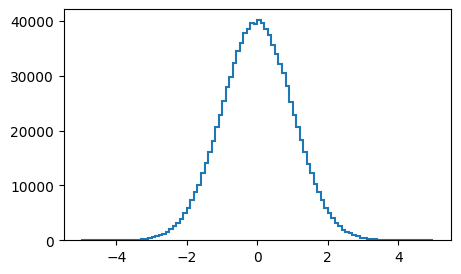
\includegraphics{./img/yamauchi_norm.png}
  \caption{山内の近似式に従って乱数を振ってみた結果}
\end{figure}

\begin{minted}
[frame=lines,
framesep=2mm,
baselinestretch=1.2,
bgcolor=lightgray,
linenos]
{python}
def yamauchi_norm():
    y = np.random.rand()
    z = -1 * np.log(4*y*(1-y))
    w = np.sqrt( z * (2.0611786 - 5.7262204/(z+11.640595)) )
    if y < 0.5 : return -1*w
    else : return w 

samples = [yamauchi_norm() for _ in range(1000000)]
fig, ax = plt.subplots(figsize=(5,3))
ax.hist(samples, bins=100, range=(-5,5), histtype="step", linewidth=1.5)
plt.show()
\end{minted}

\subsection{幾何分布}

幾何分布
\begin{equation}
  P(X=n) = p(1-p)^{1-n}
\end{equation}
の指数分布の分布関数は、初項 $p$、公比 $1-p$ の等比数列であることに留意して
\begin{eqnarray}
  F(X=n) &=& \sum_{k\leq n} P(X=k) \\ 
  &=& \sum p(1-p)^{1-k}\\
  &=& 1-(1-p)^n
\end{eqnarray}
となる。
逆関数法を用いるために
\begin{eqnarray}
  1-(1-p)^{n-1} &<& U \leq 1-(1-p)^n \\
  -(1-p)^{n-1} &<& U-1 \leq (1-p)^n \\
  (1-p)^{n} &\leq& U-1 < (1-p)^{n-1} \\
  (1-p)^{n} &\leq& U < (1-p)^{n-1}
\end{eqnarray}
として(最後の変形では $1-U\to U$の置き換えを、これまで同様に行った)、これを満たす $n$ を
$X$ 値とすれば良い。

\section{ガンマ分布}

ガンマ分布の確率密度関数は
\begin{equation}
  f(x) = \frac{1}{\lambda \Gamma(\alpha)} \left(\frac{x}{\lambda}\right)^{\alpha-1} e^{-x/\lambda}
\end{equation}
であり、$Ga(\alpha,1/\lambda)$ で表される\footnote{教科書p.17と$\lambda$の意味が異なることに留意。}。
$\alpha$は形状パラメータ、$\lambda$は尺度パラメータと呼ばれるパラメータである。

ガンマ分布に従う乱数生成の際に、形状パラメータ $\alpha$ が整数・半整数か、それ以外かで生成の方法が異なる。

\subsection{形状パラメータが整数・半整数のとき}
\subsubsection{形状パラメータが整数のとき}
ガンマ分布 $G(1,1/\lambda)$ は
\begin{equation}
  Ga(1,1/\lambda) = \frac{1}{\lambda} e^{-x/\lambda}
\end{equation}
となり、期待値 $\lambda$ の指数分布に等しい。指数乱数の生成方法と同様に、$Ga(1,1/\lambda)$ に従う乱数は
\begin{equation}
  X_1 = -\lambda \log U_1
\end{equation}
と与えられる。またガンマ分布の再生性から、共通の尺度パラメータを持っていれば
\begin{equation}
 X_1 + X_2 \sim G(\alpha_1+\alpha_2,1/\lambda) 
\end{equation}
であるので、
\begin{equation}
  X = -\lambda\log U_1  -\lambda\log U_2 + ... -\lambda\log U_n = -\lambda \log U_1U_2...U_n
\end{equation}
は $G(n,1/\lambda)$ に従うガンマ乱数を与えることになる。

\subsubsection{形状パラメータが半整数のとき}
形状パラメータが半整数のときには、$2/\lambda Z^2$ が $G(1/2,1/\lambda)$ に従うので
\begin{equation}
  X = -\lambda \log U_1U_2...U_n + (\lambda/2) Z^2
\end{equation}
が $GA(n+1/2,1/\lambda)$ に従うガンマ乱数を与える。


\subsection{ポワソン分布}

$X_1,X_2,X_3... \sim Ex(\lambda)$ ならば
\begin{equation}
  Y = \sup \{n~|~X_1+X_2+...+X_n \leq 1\}
\end{equation}
はパラメータ $\lambda$ のポワソン分布に従う。指数乱数は逆関数法で作成すると
\begin{eqnarray}
  -\frac{1}{\lambda} \log U_1 - \frac{1}{\lambda} \log U_2 - ... &<& 1 \\
  \log U_1 +  \log U_2 + ... &>& -\lambda \\
  U_1U_2...U_n &>& e^{-\lambda}
\end{eqnarray}
で与えられる。



\end{document}
